\section[Mathematical Model]{Mathematical Model}
\label{Mathematical_Model}

We propose a Mixed-Integer Linear Programming (MILP) model to solve the problem. First, in Section~\ref{graph-modeling}, we illustrate in detail how to construct a graph representing the spatio-temporal permits shared by the drones.

\subsection{Graph Modeling} \label{graph-modeling}

Following the flow network problem paradigm, we model our spatio-temporal permits as a directed graph (digraph) $G = (V, A)$, where:

\begin{itemize}
  \item $V$ is the set of nodes representing the airspace and virtual drone locations.
  \item $A$ is the set of directed arcs representing the permitted transitions between nodes.
\end{itemize}

The temporal component is omitted here as we are primarily interested in representing the problem's spatial topology.

\begin{figure}[H]
  \centering
  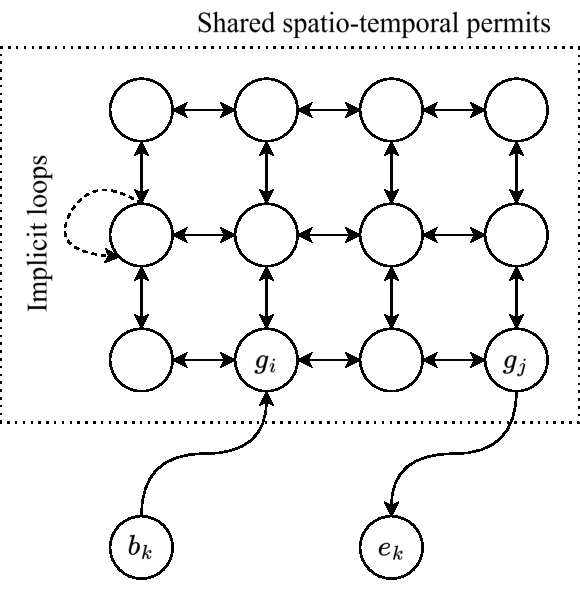
\includegraphics[width=0.8\textwidth]{img/graph_model.pdf}
  \caption[graph modelling]{Graph modelling. Source: The authors.}
  \label{fig:graph_model}
\end{figure}



Figure~\ref{fig_graph} depicts a simplified 2D grid-shaped example of a shared airspace (without altitude) for illustrative purposes. The dotted rectangular area represents the physical 2D airspace.

\subsubsection{Virtual Nodes for Drones}

In addition to the shared airspace, we introduce two virtual nodes for each drone $k$:

\begin{itemize}
  \item A source node $b_k$: This represents the starting point of drone $k$'s mission.
  \item A sink node $e_k$: This represents the ending point of drone $k$'s mission.
\end{itemize}


Each drone $k$ must initiate its mission at $b_k$ and conclude it at $e_k$. These virtual nodes streamline the model by circumventing the need to explicitly handle individual drone start and end positions.

Here's a breakdown of the virtual node connections:

\begin{itemize}
  \item Drone $k$ can only remain in $b_k$ or exit it to the shared airspace.
  \item Once exited, no drone (including $k$ itself) can re-enter $b_k$.
  \item A priori, any drone $k$ can enter its designated sink node $e_k$. However, constraints will be formulated in the mathematical programming section to ensure only drone $k$ enters its corresponding $e_k$.
\end{itemize}

\subsubsection{Drone Loitering}

Since we're dealing with rotary-wing vehicles, the model allows drones to remain (loiter) at a node for a certain time. To accommodate this, we include a loop arc for every node in the graph, encompassing both physical and virtual source/sink nodes. For clarity, these loops are implicitly considered in the example of Figure~\ref{fig_graph} and not explicitly depicted.

Including loops simplifies the mathematical programming model by avoiding the need to address potential exceptions.

\subsection{Parameters}

Below are listed the parameters that are constants of the problem:

\begin{itemize}
\item $T$: maximum time allowed for the mission (limits drone movement);
\item $b_k$: initial virtual vertex representing the initial position (begin) of drone $k$;
\item $e_k$: final virtual vertex representing the final position (end) of drone $k$;
\item $\mathcal{R}$: set of drones;
\item $\mathcal{G}$: digraph $(\mathcal{V}, \mathcal{A})$ representing the airspace;
\item $\mathcal{V}$: set of vertices of $\mathcal{G}$ representing each cell of the airspace or virtual vertex;
\item $\mathcal{B} \subset \mathcal{V}$: set of initial virtual vertices $b_k$;
\item $\mathcal{E} \subset \mathcal{V}$: set of final virtual vertices $e_k$;
\item $\mathcal{S}$: set $\mathcal{V} \setminus (\mathcal{B} \cup \mathcal{E})$ of vertices exclusively representing the shared airspace, i.e., eliminating virtual vertices;
\item $\mathcal{A}$: set of arcs $(i,j) \in \mathcal{A}$ of $\mathcal{G}$ connecting airspace cells to each other or a virtual vertex to the airspace.
\end{itemize}

\subsection{Indices}

In the equations, we use the following iteration indices:

\begin{itemize}
\item $k$ : drone $\implies$ $k \in \mathcal{R}$;
\item $t$ : time $\implies$ $1 \leq t \leq T $;
\item $i,j,l$ : vertices $\implies$ $i, j, l \in \mathcal{V}$.
\end{itemize}

\subsection{Decision Variables}

Below are listed the decision variables of the model:

\begin{itemize}
\item $x_{i,j,t}^k = 1 \iff$ drone $k$ jumps from $i$ to $j$ at time $t$.
\end{itemize}


\subsection{Objective Function}

We choose an objective function that minimizes the total sum of the number of drone movements,
\begin{equation}\label{eq:fobj}
\min
\sum_{k \in \mathcal{R}}
\sum_{t=1}^T
\sum_{ \; (i,j) \in \mathcal{A}:\ j \notin (\mathcal{E} \cup \mathcal{B})} x_{i,j,t}^{k}\text{,}
\end{equation}
counting $n-1$ jumps for each drone that performs $n$ jumps, since the jump to the final virtual vertex cannot be counted as a vertex with cost for the drone mission. Loops at initial virtual vertices are also disregarded.

\subsection{Constraints}

The set of constraints are described in the following.

\subsubsection{Movement Start}

We require that each drone starts its mission, \begin{equation}\label{eq:restr_inicio}
\sum_{t=1}^{T}
\sum_{j \in \mathcal{S}}
x_{b_k,j,t}^k = 1, \quad \forall k \in \mathcal{R}
\end{equation},  by jumping from its virtual initial node $b_k$ to the shared airspace.

\subsubsection{Flow Conservation}

 The flow conservation is also addressed,  \begin{equation}\label{eq:restr_fluxo}
\sum_{j \in \mathcal{V}} x_{i,j,t-1}^{k} =
\sum_{l \in \mathcal{V}} x_{j,l,t}^{k}, \quad
\forall j \in \mathcal{V}, \forall k \in \mathcal{R}, \forall t \in \{2, \ldots, T\} \; \text{,}
\end{equation} ensuring the consistency of allowed movements defined by the graph $\mathcal{G}$

\subsubsection{Border Condition}

Initially, under the border condition at time $t=0$, we consider there is a loop flow of drones at the virtual initial vertices.
This flow is redirected into the problem by the flow conservation constraint. \begin{equation}\label{eq:restr_borda}
    x_{i,j,0}^k = \left\{
    \begin{matrix}
        1, & \text{if}\ i=b_k \land j=b_k,\\
        0, & \text{otherwise}.
    \end{matrix}
    \right.
    \quad \forall k \in \mathcal{R}, \forall (i,j) \in A  \; \text{.}
\end{equation} For all other variables at time $t=0$, we consider a flow equal to zero.

\subsubsection{Mutual exclusion of vertex occupation}

We ensure that no drones occupy the same position,

\begin{equation}\label{eq:restr_ocupacao}
\sum_{k \in \mathcal{R}}
\sum_{j \in \mathcal{V}}
x_{i,j,t}^{k} \leq 1, \quad \forall j \in \mathcal{V}, \forall t \in \{1, \ldots, T\} \; \text{,}
\end{equation} that is, each vertex $j \in \mathcal{V}$ is occupied by at most one drone.

\subsubsection{Mission Accomplishment}

Every drone $k$ needs to complete its mission, 

\begin{equation}\label{eq:restr_fim}
\sum_{t=1}^{T}
\sum_{i \in \mathcal{S}}
x_{i,e_k,t}^k \geq 1, \quad \forall k \in \mathcal{R} \; \text{,}
\end{equation} i.e., reaching its final virtual vertex $e_k$ is required.
